%%
%% This is file `sample-sigchi.tex',
%% generated with the docstrip utility.
%%
%% The original source files were:
%%
%% samples.dtx  (with options: `sigchi')
%% 
%% IMPORTANT NOTICE:
%% 
%% For the copyright see the source file.
%% 
%% Any modified versions of this file must be renamed
%% with new filenames distinct from sample-sigchi.tex.
%% 
%% For distribution of the original source see the terms
%% for copying and modification in the file samples.dtx.
%% 
%% This generated file may be distributed as long as the
%% original source files, as listed above, are part of the
%% same distribution. (The sources need not necessarily be
%% in the same archive or directory.)
%%
%% The first command in your LaTeX source must be the \documentclass command.
\documentclass[sigchi]{acmart}
%\documentclass[manuscript,screen]{acmart}
%\usepackage [slovene]{babel}
\usepackage[T1]{fontenc}
\usepackage[pdftex]{graphicx}
\usepackage[utf8]{inputenc}

%%
%% \BibTeX command to typeset BibTeX logo in the docs
\AtBeginDocument{%
  \providecommand\BibTeX{{%
    \normalfont B\kern-0.5em{\scshape i\kern-0.25em b}\kern-0.8em\TeX}}}

%% Rights management information.  This information is sent to you
%% when you complete the rights form.  These commands have SAMPLE
%% values in them; it is your responsibility as an author to replace
%% the commands and values with those provided to you when you
%% complete the rights form.
%\setcopyright{none}
%\setcopyright{acmcopyright}
%\copyrightyear{2018}
%\acmYear{2018}
%\acmDOI{10.1145/1122445.1122456}

%% These commands are for a PROCEEDINGS abstract or paper.
%\acmConference[Woodstock '18]{Woodstock '18: ACM Symposium on Neural
%  Gaze Detection}{June 03--05, 2018}{Woodstock, NY}
%\acmBooktitle{Woodstock '18: ACM Symposium on Neural Gaze Detection,
%  June 03--05, 2018, Woodstock, NY}
%\acmPrice{15.00}
%\acmISBN{978-1-4503-9999-9/18/06}

%%
%% Submission ID.
%% Use this when submitting an article to a sponsored event. You'll
%% receive a unique submission ID from the organizers
%% of the event, and this ID should be used as the parameter to this command.
%%\acmSubmissionID{123-A56-BU3}

%%
%% The majority of ACM publications use numbered citations and
%% references.  The command \citestyle{authoryear} switches to the
%% "author year" style.
%%
%% If you are preparing content for an event
%% sponsored by ACM SIGGRAPH, you must use the "author year" style of
%% citations and references.
%% Uncommenting
%% the next command will enable that style.
%%\citestyle{acmauthoryear}

%%
%% end of the preamble, start of the body of the document source.
\begin{document}

%%
%% The "title" command has an optional parameter,
%% allowing the author to define a "short title" to be used in page headers.
\title[Sound 2121: Cross-Reality Sound Transitions]{Sound 2121: Cross-Reality Transitions Between Real and Augmented Sound Landscapes}


%switching between music listening and the environment sounds}


%%
%% The "author" command and its associated commands are used to define
%% the authors and their affiliations.
%% Of note is the shared affiliation of the first two authors, and the
%% "authornote" and "authornotemark" commands
%% used to denote shared contribution to the research.

\author{Jordan Aiko Deja}
\email{jordan.deja@famnit.upr.si}
\affiliation{%
  \institution{University of Primorska, UP FAMNIT}
  \streetaddress{Glagoljaška 8}
  \city{Koper}
  \state{Slovenia}
  \postcode{SI-6000}
}

\author{Nuwan T. Attygale}
\email{nuwan.attygalle@upr.si}
\affiliation{%
  \institution{University of Primorska, UP FAMNIT}
  \streetaddress{Glagoljaška 8}
    \city{Koper}
  \state{Slovenia}
  \postcode{SI-6000}
}

\author{Klen Čopič Pucihar}
%\authornotemark[1]
\email{klen.copic@famnit.upr.si}
\affiliation{%
  \institution{University of Primorska, UP FAMNIT}
  \streetaddress{Glagoljaška 8}
  \city{Koper}
  \state{Slovenia}
  \postcode{SI-6000}
}
\affiliation{%
  \institution{Faculty of Information Studies}
  \streetaddress{Ljubljanska cesta 31a}
  \city{Novo mesto}
  \state{Slovenija}
  \postcode{SI-8000}
}

\author{Matjaž Kljun}
\email{matjaz.kljun@famnit.upr.si}
\orcid{1234-5678-9012}
\affiliation{%
  \institution{University of Primorska, UP FAMNIT}
  \streetaddress{Glagoljaška 8}
  \city{Koper}
  \state{Slovenia}
  \postcode{SI-6000}
}
\affiliation{%
  \institution{Faculty of Information Studies}
  \streetaddress{Ljubljanska cesta 31a}
  \city{Novo mesto}
  \state{Slovenija}
  \postcode{SI-8000}
}

\renewcommand{\shortauthors}{J. A. Deja, N. T. Attygale, K. Čopič Pucihar, M. Kljun}
\settopmatter{printacmref=false}

\begin{abstract}
Music and sounds have always been an integral part of our society since the prehistoric times. However, music listening has moved from a social experience to a more personal one with audio systems such as speakers moving ever closer to our ear canal. Based on this pattern and various futuristic visions of how we are going to listen to music, one can start to imagine a situation where a chip in our auditory cortex will stream sounds directly to our brain. However, augmenting our hearing with objects around us capable of streaming sounds directly to our brains might exacerbate the already present problem of blocking the environment sounds and not paying attention to what is happening around us. In this positional paper we discuss not only ``What is the future of music listening and how will we consume music a hundred years from now?'' but also ``How are we going to enable users to pay attention to their environment and enjoy music listening at the same time?'' Put differently, how are we enabling users to constantly switch between the real and augmented sound landscapes and enable seamless cross-reality transitions as well as preserve a positive user experience. 
\end{abstract}

%%
%% The code below is generated by the tool at http://dl.acm.org/ccs.cfm.
%% Please copy and paste the code instead of the example below.
%%
%\begin{CCSXML}
%<ccs2012>
%   <concept>
%       <concept_id>10003120.10003123.10011758</concept_id>
%       <concept_desc>Human-centered computing~Interaction design theory, concepts and paradigms</concept_desc>
%       <concept_significance>500</concept_significance>
%       </concept>
% </ccs2012>
%\end{CCSXML}

%\ccsdesc[500]{Human-centered computing~Interaction design theory, concepts and paradigms}
%%
%% Keywords. The author(s) should pick words that accurately describe
%% the work being presented. Separate the keywords with commas.
\keywords{music listening, brain-chip interface, sound streaming, future vision}

%% A "teaser" image appears between the author and affiliation
%% information and the body of the document, and typically spans the
%% page.
\begin{teaserfigure}
  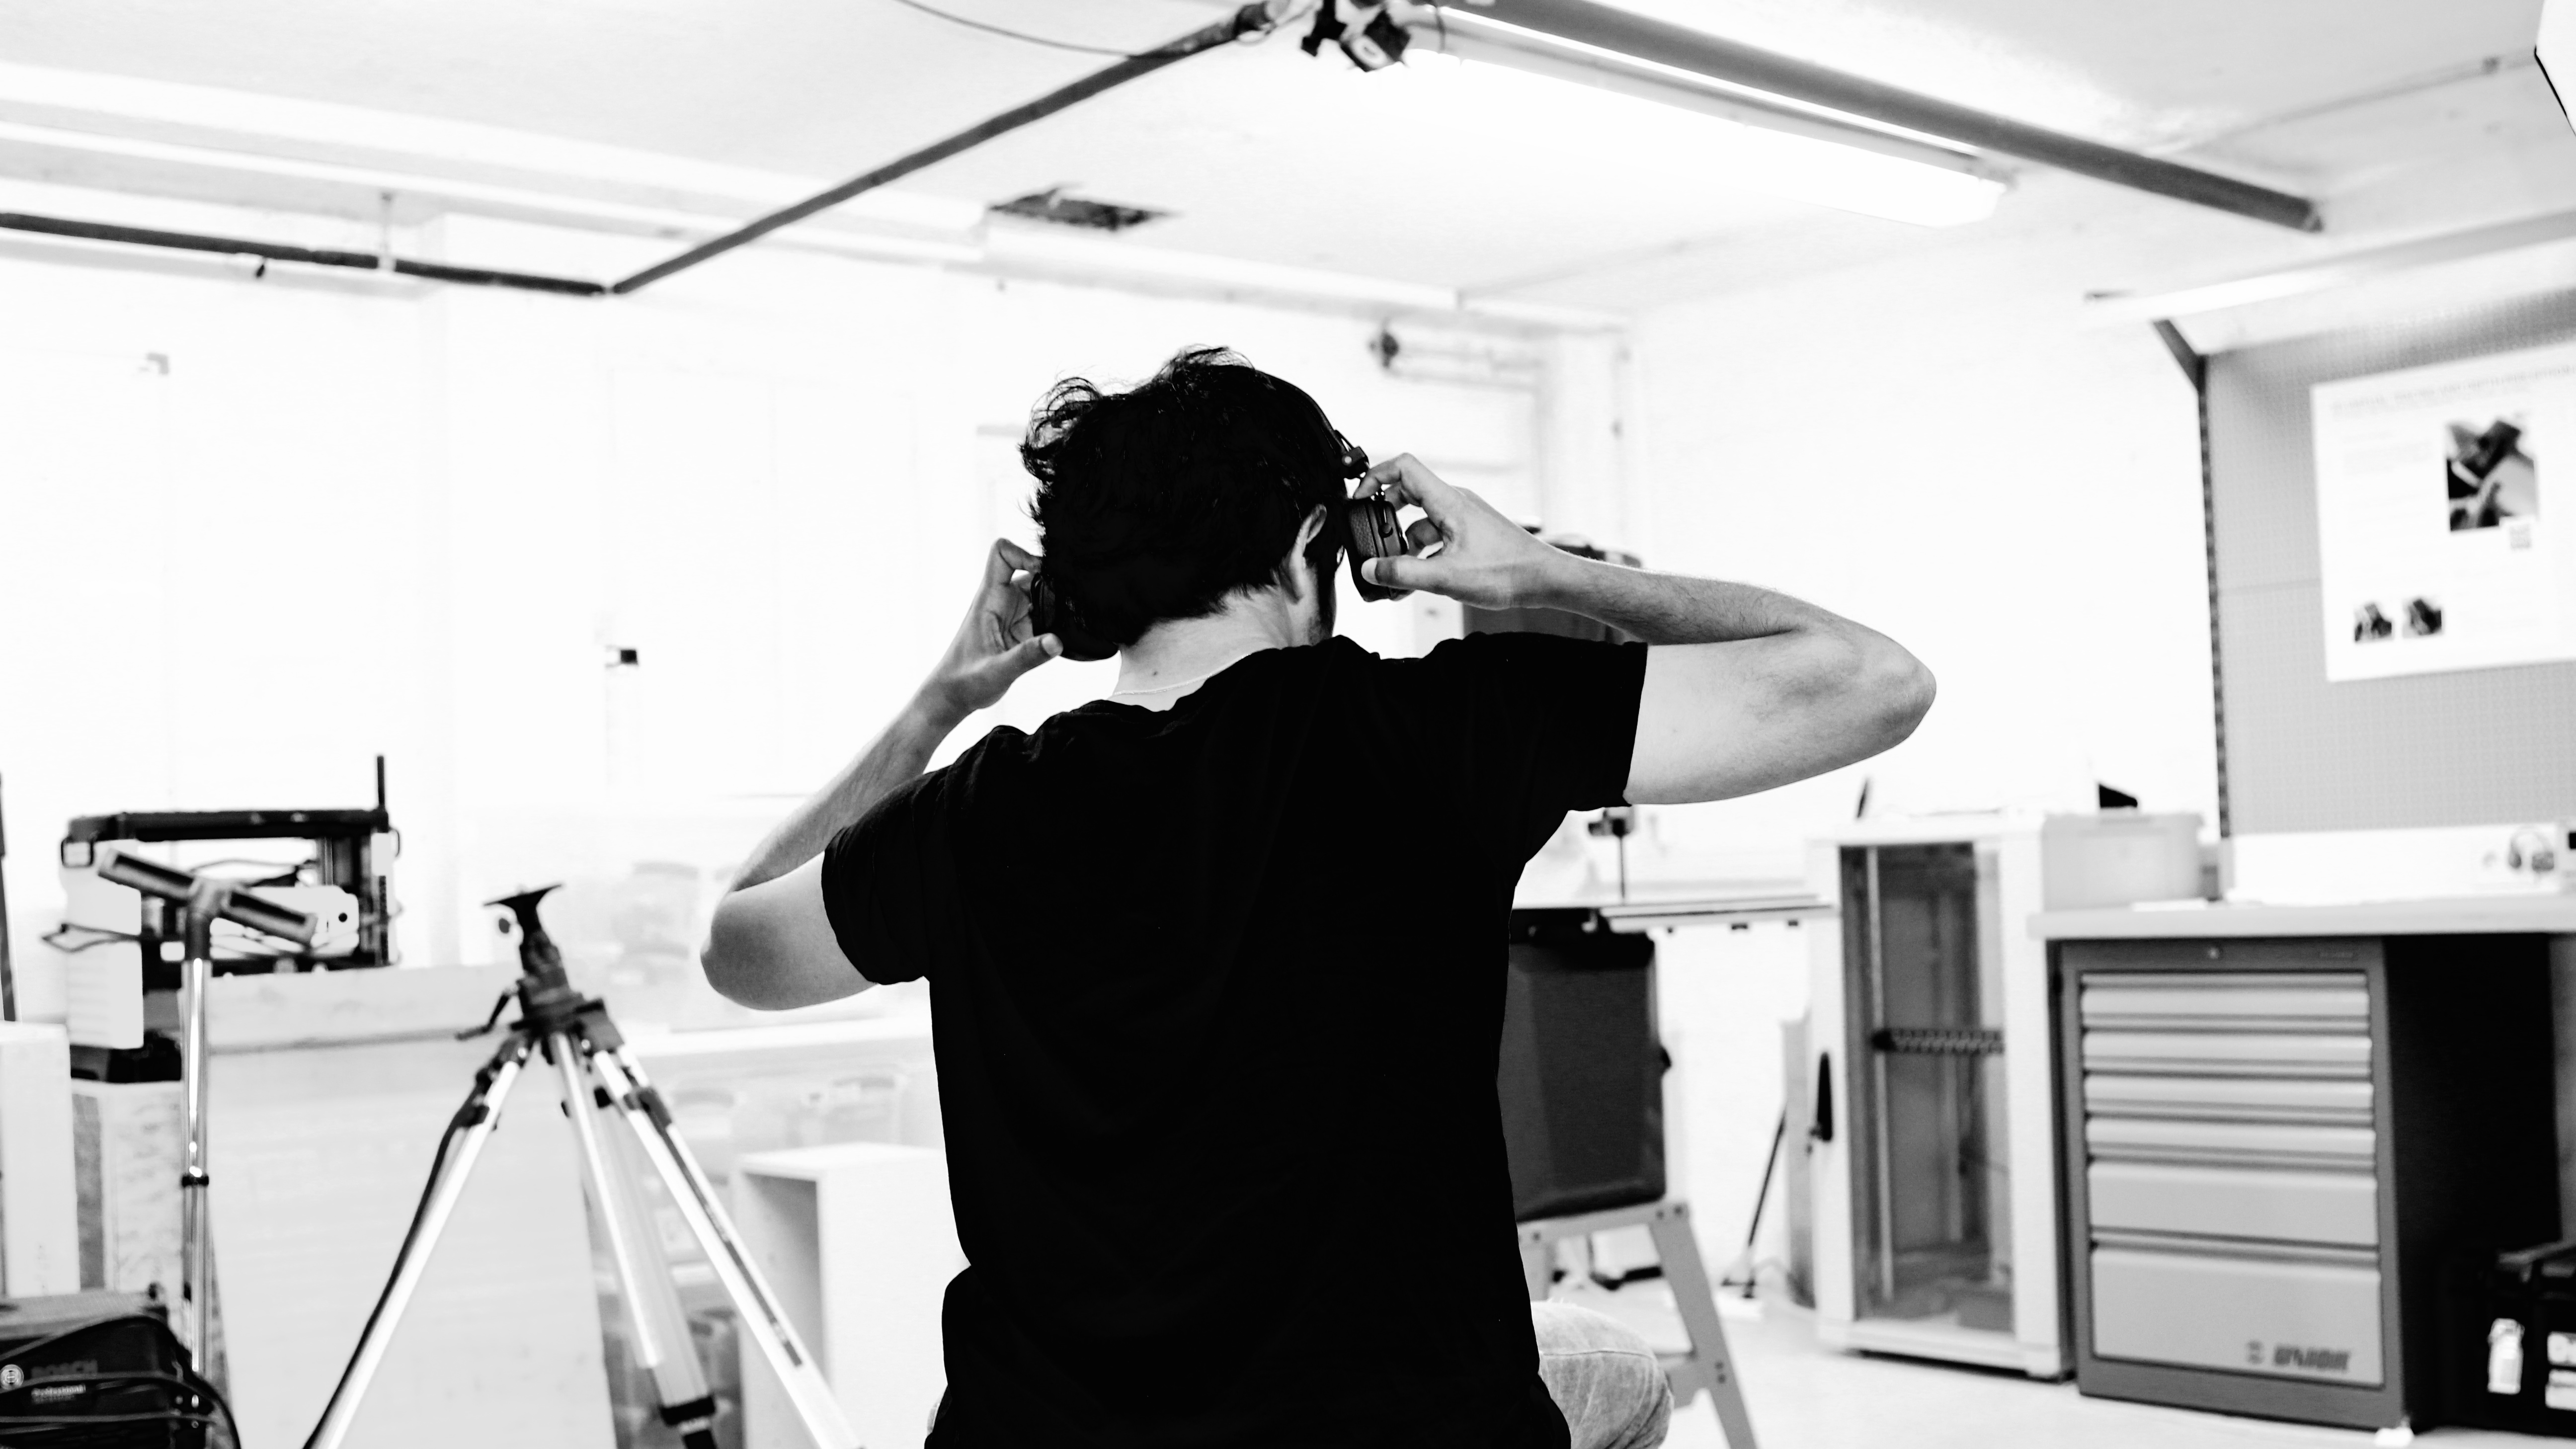
\includegraphics[trim={0 5.5cm 0 3.5cm}, clip, width=\textwidth]{acmart-master-2/samples/test2bw.png}
  \caption{Concept: Envision a future where we no longer need tangible interfaces to listen to music but stream it directly into our auditory cortex. How do we enable seamless transition between environment and augmented streamed sounds in such scenario?}
  \Description{photo of a user removing headphones.}
  \label{fig:teaser}
\end{teaserfigure}
%%
%% This command processes the author and affiliation and title
%% information and builds the first part of the formatted document.
\maketitle

One area of Cross-Reality (XR) Interaction %\footnote{https://xr.famnit.upr.si} 
explores the shift between multiple systems on the Milgram's reality-virtuality continuum. % or the concurrent usage in between these systems that may or may not entirely diminish the distinction of both Augmented Reality (AR) and Virtual Reality (VR). 
In this position paper, we envision a future with a chip-to-brain sound transmitting interface that allows interaction between and mixing of multiple sound realities and virtualities from the environment sound to music listening. Our position diverts from the typical visual augmented and virtual reality but rather focuses on the problems of sound and how humans transition between different sound sources. We intend to share a perspective that may consider also the transitions induced by visual elements, augmentations and virtual worlds as they are consumed with sound. This paper also encourages several questions such as how to retain users' attention, task-awareness and even social communication while interacting with the environmental sound as well as streamed one (be it from digital objects in the environment or unrelated to the environment such as listening to music). 


%\section{Music listening throughout history}

\section{Introduction}

Music is considered to be culturally universal \cite{campbell1997music, seeger1971reflections} and present across all parts of the globe, reshaping the ways human live, express themselves and convey emotions \cite{juslin2001music,montagu2017music}. It is believed that music originated from naturally occurring sounds and rhythms that humans echoed by merging them in patterns, making repetitions while changing tonality using their voice~\cite{montagu2017music, morley2013prehistory}, hands clapping \cite{kassler1987dancing}, and smacking stones, sticks and other objects around them \cite{montagu2014horns}. Music has also helped humans in terms of survival, forging a sense of group identity and mutual trust \cite{conard2009new}. 

We create and consume music for various purposes including: (i) dancing as a social exercise, (ii) providing a common form of personal or community entertainment, (iii) communicating ideas and emotions and (iv) having and celebrating rituals and other activities \cite{montagu2017music}. While these purposes come in handy for a variety of music activities, this positional paper is focusing on music listening only, which is present in (i) where listening is a shared experience, and in (ii) and (iv) where listening can be a shared as well as a personal experience. 

In the past, human tribes gathered around fires where one or several members of the group performed a music piece singing and playing instruments. This type of ``community entertainment'' or ``celebrations'' has been present for a long period of time and even nowadays people gather in live concerts, events and rituals to collectively listen to music. With recordings and radio, music has moved to people's homes and the collective listening has been reduced to family members, friends or an individual (we do not count all the radio audience towards this group since listeners are not co-present~\cite{bonini2014new}). Nevertheless, the sounds were still coming from the speaker(s) in our environment and listening to the radio was often a social event. The headphones enabled users to experience music individually and the Walkman enabled us to do it on-the-go. Smartphones and internet have expanded the instant availability of music but the consumption remained mainly personal. Looking at how listening to music has moved closer and closer to our ear canal with in-ear headphones, it is not far-fetched if we envision that listening to music will move inside our heads.

\section{Re-imagining music listening interface}

%\begin{figure}[h]
%  \centering
%   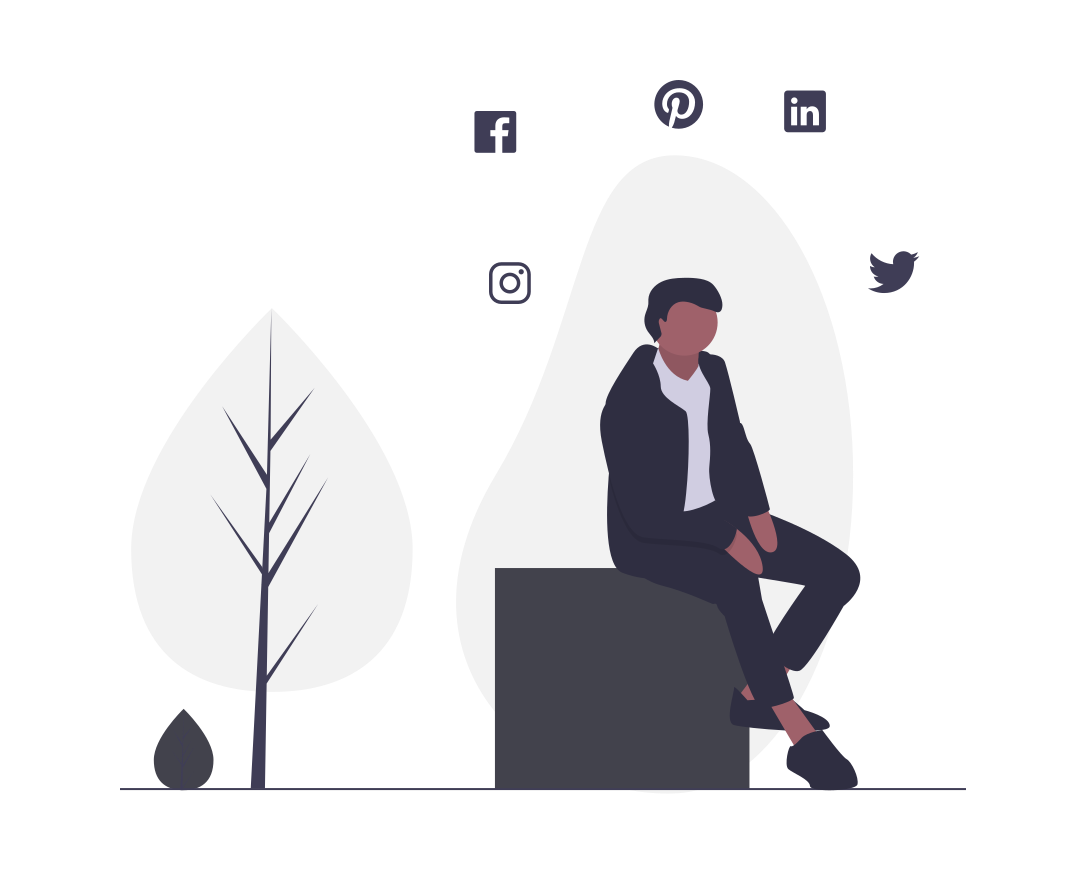
\includegraphics[width=\linewidth]{acmart-master-2/samples/thinkbnw.png}
%  \caption{Concept: Humans do not need tablets, mobile devices, or digital walls. Ideas and concepts are conceived in and are played into our brains from the surrounding objects.}
%  \Description{Figure of a person thinking and not touching anything.}
%  \label{fig: think}
%\end{figure}

Having a chip in our brain seems like a far fetched idea but several researchers are working on enabling people with impairments to interact with computers and the world around them via implanted chips~\cite{santhanam2006high}. A recent startup Neuralink\footnote{https://neuralink.com/} envisions all humans to have such a chip in order to interact with smart devices around us. However, for many, implanting a chip in our brain is not appealing at the moment~\cite{metz2019chipbrain}. Nevertheless, as privacy boundary with the advent of social media has risen or using mobile phones in restaurants has become a norm, what is individually and culturally accepted is rapidly changing. This shows that technologies are moving forward far quicker than societal ability to grasp all moral and legal implications they are introducing.

The vision of ``the always on'' streaming music (and other sounds) to our brain via a chip on the biological and psychological level adapting based on our mood on the fly is not new. Such neurological interface instead of a visual or voice one has been envisioned before~\cite{cherie2019bravenewworld}. With researchers and futurists working on biometric recommendation systems~\cite{zhang2018system} we could potentially achieve this in the near future. At the moment, the company called Weav\footnote{https://www.weav.io/} is already adapting music rhythm to the heartbeat ``augmenting and intensifying the listening experience at all levels''. 

This envisioned streaming interface will be supported by the internet of things (IoT) vision with biological and artificial objects around us connected \cite{weisman2004internet} and having access to a superb computing power. These devices will not only be able to stream music, but also produce their own sounds, melodies, and rhythms or augment the existing ones. Besides physical objects in the physical environment, there might be a plethora of virtual objects around us as well that will communicate with us not only visually but also vocally.

Despite all these visions and developments, we still have not solved the issues related to current music consumption over the headphones. One of such issues is enabling users to hear sounds from the environment (be it from physical or virtual objects and environments) while still enjoying their music. 

\section{Switching between the environment sound to augmented streamed one}

Today's headphones are complex small devices that are capable of actively and passively cancelling environment noise in order to enable users to be uninterrupted while listening to the their favourite tunes. In-ear buds even mechanically block outer sounds from entering the auditory canal. While these might be desirable features on some occasions they are also problematic since the sounds from the environment provide a cue of what is happening around us and humans always relied on these sounds in order to survive. The sounds of objects around us are even nowadays so important for our safety that legislators made it obligatory for electric cars to make artificial engine noise~\cite{guy2019carnoise}. Even some electric go-karts have introduced gas engine noise to make the experience more immersive and believable. However, seeing a cyclist, pedestrian or a car driver with the headphones is not an unusual sight and greatly affects users' situational awareness~\cite{roads2018headphonedriving}. 


How do we then switch or transition between the envisioned future ``always on, always-adaptive'' music streaming into our auditory cortex provided by the IoT enabled devices and the environment sound in order to increase our safety or enable social interaction? 

Music is also vibration; for example, it has been noted that the part of the brain responsible for hearing, works perfectly in deaf people as well \cite{abcsciencemusic}. In order to ``hear'' music, we do not need to actually hear it but rather receive the stimulus to the hearing region of the brain. This has for example been explored in bone conduction ``headphones'' conducting sound to the inner ear primarily through the bones of the skull. Some consumer products already use this technology such as Google Glass and BAE helmet. The latter for example enabled a sailing crew in the 2017 America's cup ``to keep both their ears free in order to hear external sounds, whilst providing the ability to communicate clearly with crewmates in the most treacherous of sailing conditions''~\cite{bae2019boneconhelmet}. A recent study also revealed that bone conduction headphones do not significantly affect driving performance or story comprehension and were no more distracting than regular car speakers \cite{granados2018usability}. This means that it is possible to mix digital sounds with the environment sounds. However, it remains unanswered how enjoyable is listening to music with such devices. 

Based on the future IoT vision with biological and artificial objects around able to communicate with each other and us, we can envision such IoT the environment to be constantly on the guard and aware of potential risks to the people in vicinity. Thus, such environment will be able to inform us in the same way it will stream sounds to our brain. Similar to the vision of autonomous cars communicating with each other and broadcast potential risks and road conditions~\cite{shankland20195gcars}. 

Since music has helped humans throughout the history in terms of survival, forging a sense of group identity and mutual trust, and since environment sound landscape helped us being alert and safe we need to enable their roles in the future as well. Be it in physical environment or in any mix of reality and virtuality. At the same time we need to avoid the ``polluted'' sound landscape as in the video of the hyper-reality vision of the future~\cite{matsuda2016hyperreality} visible on Figure~\ref{fig:hyper-reality} where adverts and services seek our attention via visuals as well as sounds. And imagine receiving these through our brain-chip interface and transitioning between the reality only and hyper-reality. 

\begin{figure*}[hbt!]
  \centering
   \includegraphics[width=\textwidth]{hyper-reality.png}
  \caption{Hyper-reality vision of the future where physical and virtual objects emit a variety of sounds and provide a cacophony of attention seeking visual and sound elements of the environment~\cite{matsuda2016hyperreality}.}
  \Description{Future environment with physical and virtual objects.}
  \label{fig:hyper-reality}
\end{figure*}

How to avoid the mentioned sound ``pollution'' and achieve smooth transitions between the augmented and environment sound landscapes and vice versa to maintain enjoyable music listening user experience as well as user safety remains to be answered when such devices will be available. 
\balance

%\section{Conclusion}

%DO WE NEED ONE KLEN?

%The visions and scenarios we presented come with their respective issues and challenges in implementation and in policy design. If we imagine a natural and seamless interface, evaluating its usability will introduce a new paradigm for HCI researchers. Will existing models such as Fitts' Law (which has always worked on any interface developed - mechanical, digital, virtual) still work in neurological links managed by our seamless thoughts? The intangible interaction provided by this \textit{"online network"} could potentially blur concepts such as piracy and intellectual property. As music is composed by ubiquitous algorithms connected to our personal thoughts and feelings, are all our emotions and the music that are generated by them considered unique? shareable? These among many others are interesting questions that we leave to our readers as we re-imagined a natural music interface. While these visions appear to be very far from reality, we are only left with our own thoughts to begin with and maybe hopefully in the not so near future too. 

\bibliographystyle{ACM-Reference-Format}
\bibliography{sample-base}

\end{document}
\endinput
%
